\chapter{函数}

\section{函数}

\subsection{函数(Function)}

数学中的函数$ y = f(x) $,通过输入$ x $的值,经过计算可以得到$ y $的值。计算机中的函数也是如此,将输入传给函数,经过处理后,会得到输出。\\

函数是一段可重复使用的代码,做了一个特定的任务。例如print()和len()就是函数,其中print()的功能是输出字符串,len()的功能是计算序列的长度。\\

\begin{figure}[H]
	\centering
	\begin{tikzpicture}[scale=0.5]
		\draw[-] (5,-2) -- (10,-2) -- (10,2) -- (5,2) -- (5,-2);
		\draw[->] (0,0) -- (5,0);
		\draw[->] (10,0) -- (15,0);

		\draw (-2,0) node {Input};
		\draw (17,0) node {Output};
		\draw (7.5,0) node {Function};
	\end{tikzpicture}
	\caption{函数}
\end{figure}

除了这些内置的函数以外,开发者还可以自定义函数,将程序中会被多次使用的代码或做了一件特定的任务的代码写成一个函数,这样就能避免重复写相同的代码,提高开发效率,也利于维护。\\

在编写函数时需要:

\begin{enumerate}
	\item 确定函数的功能
	      \begin{itemize}
		      \item 函数名
		      \item 确保一个函数只做一件事
	      \end{itemize}

	\item 确定函数的输入(参数)
	      \begin{itemize}
		      \item 是否需要参数
		      \item 参数个数
		      \item 参数类型
	      \end{itemize}

	\item 确定函数的输出(返回值)
	      \begin{itemize}
		      \item 是否需要返回值
		      \item 返回值类型
	      \end{itemize}
\end{enumerate}

\vspace{0.5cm}

\mybox{最大值}

\begin{lstlisting}[language=Python]
def max(num1, num2):
    # if num1 > num2:
    #     return num1
    # else:
    #     return num2

    return num1 if num1 > num2 else num2

print(max(4, 12))
print(max(54, 33))
print(max(-999, -774))
\end{lstlisting}

\begin{tcolorbox}
	\mybox{运行结果}
	\begin{verbatim}
12
54
-774
	\end{verbatim}
\end{tcolorbox}

函数也可以没有返回值,因为它执行完函数后,并不需要将结果返回给调用者。\\

\mybox{棋盘}

\begin{lstlisting}[language=Python]
def print_board():
    for i in range(3):
        for j in range(2):
            print("   |", end='')
        print()
        if i < 2:
            print("---+---+---")

print_board()
\end{lstlisting}

\begin{tcolorbox}
	\mybox{运行结果}
	\begin{verbatim}
   |   |
---+---+---
   |   |
---+---+---
   |   |
	\end{verbatim}
\end{tcolorbox}

\vspace{0.5cm}

\subsection{函数调用}

当调用函数时,程序会记录下当前的执行位置,并跳转到被调用的函数处执行。当被调用的函数执行结束后,程序会回到之前的位置继续执行。\\

\begin{figure}[H]
	\centering
	\begin{tikzpicture}[]
		\draw (0,4.5) node {Caller};
		\draw[->] (0,4) -- (0,0.5);
		\draw[->] (0,-0.5) -- (0,-4);
		\draw (0,0) node {调用foo()};

		\draw (4,4) node {foo()};
		\draw[->] (4,3) -- (4,0.5);
		\draw[->] (4,-0.5) -- (4,-3);
		\draw (4,0) node {调用bar()};

		\draw (8,3) node {bar()};
		\draw[->] (8,2) -- (8,-2);

		\draw[->] (0.5,0.5) -- (3.5,3);
		\draw[->] (3.5,-3) -- (0.5,-0.5);
		\draw[->] (4.5,0.5) -- (7.5,2);
		\draw[->] (7.5,-2) -- (4.5,-0.5);
	\end{tikzpicture}
	\caption{函数调用}
\end{figure}

\vspace{0.5cm}

\mybox{两点间距离}

\begin{lstlisting}[language=Python]
import math

def square(x):
	return x ** 2
	
def distance(point1, point2):
	x1, y1 = point1
	x2, y2 = point2
	return math.sqrt(square(x1 - x2) + square(y1 - y2))
	
x1, y1 = eval(input("Enter (x1, y1): "))
x2, y2 = eval(input("Enter (x2, y2): "))
print("Distance:", distance((x1, y1), (x2, y2)))
\end{lstlisting}

\begin{tcolorbox}
	\mybox{运行结果}
	\begin{verbatim}
Enter (x1, y1): 0, 0
Enter (x2, y2): 3, 4
Distance: 5.0
	\end{verbatim}
\end{tcolorbox}

\vspace{0.5cm}

\subsection{main()}

很多编程语言都使用main()函数作为程序的入口,在Python中main()并不是必须的,但是使用main()函数可以使代码的结构更加清晰。\\

\_\_name\_\_是一个内置变量,当文件作为程序执行时,其值为\_\_main\_\_。

\vspace{-0.5cm}

\begin{lstlisting}[language=Python]
def main():
    pass

if __name__ == "__main__":
    main()
\end{lstlisting}

\newpage

\section{作用域}

\subsection{局部变量(Local Variable)}

定义在块中的变量称为局部变量,它只能在块中访问。当代码块结束时,局部变量就会被销毁。因此,局部变量的生命周期为从声明时开始到所在块结束。\\

块与块之间的局部变量是互相独立的,即使变量名相同,它们也不是同一个变量。\\

例如在函数调用中,函数的参数也是局部变量,它们的作用域仅限于函数内。\\

例如一个用于交换两个变量的函数swap(),在main()中的变量a和b与swap()中的a和b并不是同一个变量。在调用swap()时,是将main()中的a和b的值复制给swap()中的a和b。swap()交换的是其内部的局部变量,并不会对main()中的a和b产生任何影响。\\

\mybox{局部变量}

\begin{lstlisting}[language=Python]
def swap(a, b):
    a, b = b, a
    print("swap(): a = %d, b = %d" % (a, b))

def main():
    a, b = 1, 2

    print("Before: a = %d, b = %d" % (a, b))
    swap(a, b)
    print("After: a = %d, b = %d" % (a, b))

if __name__ == "__main__":
    main()
\end{lstlisting}

\begin{tcolorbox}
	\mybox{运行结果}
	\begin{verbatim}
Before: a = 1, b = 2
swap(): a = 2, b = 1
After: a = 1, b = 2
	\end{verbatim}
\end{tcolorbox}

\vspace{0.5cm}

\subsection{全局变量(Global Variable)}

全局变量拥有比局部变量更长的生命周期,它的生命周期贯穿整个程序。全局变量可以被程序中所有函数访问。\\

全局变量一般用于:

\begin{itemize}
	\item 定义在整个程序中都会被使用到的常量(例如数组容量)
	\item 被函数间共享的变量(例如计数器)
\end{itemize}

\vspace{0.5cm}

\mybox{全局变量}

\begin{lstlisting}[language=Python]
a, b = 1, 2

def swap():
	global a, b
	a, b = b, a
	print("swap(): a = %d, b = %d" % (a, b))

def main():
	print("Before: a = %d, b = %d" % (a, b))
	swap()
	print("After: a = %d, b = %d" % (a, b))

if __name__ == "__main__":
	main()
\end{lstlisting}

\begin{tcolorbox}
	\mybox{运行结果}
	\begin{verbatim}
Before: a = 1, b = 2
swap(): a = 2, b = 1
After: a = 2, b = 1
	\end{verbatim}
\end{tcolorbox}

\newpage

\section{函数参数}

\subsection{默认参数}

函数参数可以有默认值,如果在调用函数时不指定某个参数的值,则使用默认值。默认参数必须放在参数列表的最后。\\

\mybox{日期}

\begin{lstlisting}[language=Python]
def format_date(year=1970, month=1, day=1):
	return "%04d/%02d/%02d" % (year, month, day)

def main():
    print(format_date(2022, 12, 16))
    print(format_date(2022, 12))
    print(format_date(2022))
    print(format_date())

if __name__ == "__main__":
	main()
\end{lstlisting}

\begin{tcolorbox}
	\mybox{运行结果}
	\begin{verbatim}
2022/12/16
2022/12/01
2022/01/01
1970/01/01
\end{verbatim}
\end{tcolorbox}

\vspace{0.5cm}

\subsection{可变参数}

函数允许传入任意数量的参数,可变参数包括位置可变参数和关键字可变参数。\\

位置可变参数使用*args将参数打包成一个元组。\\

\mybox{乘法}

\begin{lstlisting}[language=Python]
def multiply(*args):
    product = 1
    for arg in args:
        product *= arg
    return product

def main():
    print(multiply(1, 2, 3))
    print(multiply(4, 2, 6, 1, 2))

if __name__ == "__main__":
    main()
\end{lstlisting}

\begin{tcolorbox}
	\mybox{运行结果}
	\begin{verbatim}
6
96
\end{verbatim}
\end{tcolorbox}

关键字可变参数使用**kwargs将参数打包成一个字典。\\

\mybox{平均分}

\begin{lstlisting}[language=Python]
def get_score_info(name, **kwargs):
    info = "[%s]\n" % name
    for subject, score in kwargs.items():
        info += "%s: %d\n" % (subject, score)
    info += "Average: %.2f" % (sum(kwargs.values()) / len(kwargs))

    return info

def main():
    print(get_score_info("Alice", Python=85, Math=80))
    print(get_score_info("Bob", Java=77, Math=82))

if __name__ == "__main__":
    main()
\end{lstlisting}

\begin{tcolorbox}
	\mybox{运行结果}
	\begin{verbatim}
[Alice]
Python: 85
Math: 80
Average: 82.50
[Bob]
Java: 77
Math: 82
Average: 79.50
\end{verbatim}
\end{tcolorbox}

\newpage

\section{递归} \label{recursion}

\subsection{递归(Recursion)}

要理解递归,得先理解递归(见\ref{recursion}章节)。\\

一个函数调用自己的过程被称为递归。递归可以轻松地解决一些复杂的问题,很多著名的算法都利用了递归的思想。

\begin{figure}[H]
	\centering
	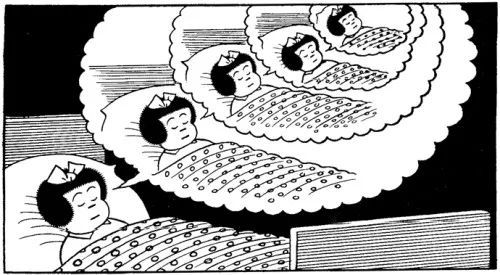
\includegraphics[scale=0.7]{img/Chapter5/5-4/1.png}
\end{figure}

\vspace{0.5cm}

\mybox{讲故事}

\begin{lstlisting}[language=Python]
def tell_story():
    story = "从前有座山,山里有座庙\n"
    story += "庙里有个老和尚\n"
    story += "老和尚在对小和尚讲故事:\n"
    print(story)

    tell_story()

def main():
    tell_story()

if __name__ == "__main__":
    main()
\end{lstlisting}

\begin{tcolorbox}
	\mybox{运行结果}
	\begin{verbatim}
从前有座山,山里有座庙
庙里有个老和尚
老和尚在对小和尚讲故事:
从前有座山,山里有座庙
庙里有个老和尚
老和尚在对小和尚讲故事:
从前有座山,山里有座庙
庙里有个老和尚
老和尚在对小和尚讲故事:
...
	\end{verbatim}
\end{tcolorbox}

一个永远无法结束的递归函数最终会导致栈溢出。因此递归函数需要确定一个结束条件,确保在递归过程中能在合适的地方停止并返回。\\

\mybox{阶乘}

\begin{lstlisting}[language=Python]
def factorial(n):
    if n == 0 or n == 1:
        return 1
    return n * factorial(n-1)

def main():
    print("5! =", factorial(5))

if __name__ == "__main__":
    main()
\end{lstlisting}

\begin{tcolorbox}
	\mybox{运行结果}
	\begin{verbatim}
5! = 120
	\end{verbatim}
\end{tcolorbox}

\begin{figure}[H]
	\centering
	\begin{tikzpicture}[]
		\draw (0,0) rectangle (3,1.5);
		\draw (3,-2) rectangle (6,-0.5);
		\draw (6,-4) rectangle (9,-2.5);
		\draw (9,-6) rectangle (12,-4.5);
		\draw (12,-8) rectangle (15,-6.5);

		\draw (12.75,-10.75) rectangle (14.25,-9.25);
		\draw (9.75,-8.75) rectangle (11.25,-7.25);
		\draw (6.75,-6.75) rectangle (8.25,-5.25);
		\draw (3.75,-4.75) rectangle (5.25,-3.25);
		\draw (0.75,-2.75) rectangle (2.25,-1.25);

		\draw (1.5,0.75) node {$ factorial(5) $};
		\draw (4.5,-1.25) node {$ factorial(4) $};
		\draw (7.5,-3.25) node {$ factorial(3) $};
		\draw (10.5,-5.25) node {$ factorial(2) $};
		\draw (13.5,-7.25) node {$ factorial(1) $};

		\draw (13.5,-10) node {$ 1 $};
		\draw (10.5,-8) node {$ 2 $};
		\draw (7.5,-6) node {$ 6 $};
		\draw (4.5,-4) node {$ 24 $};
		\draw (1.5,-2) node {$ 120 $};

		\draw[->] (3,0.75) -- (4.5,0.75) -- (4.5,-0.5);
		\draw[->] (6,-1.25) -- (7.5,-1.25) -- (7.5,-2.5);
		\draw[->] (9,-3.25) -- (10.5,-3.25) -- (10.5,-4.5);
		\draw[->] (12,-5.25) -- (13.5,-5.25) -- (13.5,-6.5);

		\draw[->] (12.75,-10) -- (10.5,-10) -- (10.5,-8.75);
		\draw[->] (9.75,-8) -- (7.5,-8) -- (7.5,-6.75);
		\draw[->] (6.75,-6) -- (4.5,-6) -- (4.5,-4.75);
		\draw[->] (3.75,-4) -- (1.5,-4) -- (1.5,-2.75);

		\draw (4.5,1) node {$ 5 * factorial(4) $};
		\draw (7.5,-1) node {$ 4 * factorial(3) $};
		\draw (10.5,-3) node {$ 3 * factorial(2) $};
		\draw (13.5,-5) node {$ 2 * factorial(1) $};

		\draw (11,-10.5) node {$ 2 * 1 $};
		\draw (8,-8.5) node {$ 3 * 2 $};
		\draw (5,-6.5) node {$ 4 * 6 $};
		\draw (2,-4.5) node {$ 5 * 24 $};
	\end{tikzpicture}
	\caption{阶乘}
\end{figure}

\vspace{0.5cm}

\mybox{斐波那契数列}

\begin{lstlisting}[language=Python]
def fibonacci(n):
    if n == 1 or n == 2:
        return n
    return fibonacci(n-2) + fibonacci(n-1)

def main():
    n = 7
    print(fibonacci(n))

if __name__ == "__main__":
    main()
\end{lstlisting}

\begin{tcolorbox}
	\mybox{运行结果}
	\begin{verbatim}
21
	\end{verbatim}
\end{tcolorbox}

\begin{figure}[H]
	\centering
	\begin{tikzpicture}[
			level distance=2.4cm,
			level 1/.style={sibling distance=6cm},
			level 2/.style={sibling distance=3cm},
			level 3/.style={sibling distance=2cm}
		]
		\node {$ f(5) $}
		child {
				node {$ f(3) $}
				child {node {$ f(1) $}}
				child {node {$ f(2) $}}
			}
		child {
				node {$ f(4) $}
				child {node {$ f(2) $}}
				child {
						node {$ f(3) $}
						child {node {$ f(1) $}}
						child {node {$ f(2) $}}
					}
			};
	\end{tikzpicture}
	\caption{递归树}
\end{figure}

递归的特点就是将一个复杂的大问题逐步简化为一个可以解决的小问题,然后再逐步计算出大问题的解。\\

递归的优点在于代码简洁易懂,但是缺点也很明显,就是效率很低。每次递归都会产生函数调用,而函数调用的开销是很大的,不适合用来解决大规模的问题。\\

例如在计算斐波那契数列的第40项时,递归需要花费大量时间,因为其中包含了大量的重复计算。相比而言,使用循环的方式能够节省大量的时间。因此像阶乘和斐波那契数列这样的情况,通常会采用循环,而不是递归进行计算。\\

然而还存在很多问题不得不使用递归的思想才能解决。\\

\mybox{阿克曼函数}

\begin{align}\nonumber
	A(m, n) =
	\begin{cases}
		n + 1             & m = 0        \\
		A(m-1, 1)         & m > 0, n = 0 \\
		A(m-1, A(m, n-1)) & m > 0, n > 0 \\
	\end{cases}
\end{align}

\begin{lstlisting}[language=Python]
def A(m, n):
    if m == 0:
        return n + 1
    elif m > 0 and n == 0:
        return A(m - 1, 1)
    else:
        return A(m - 1, A(m, n - 1))

def main():
    print(A(3, 4))

if __name__ == "__main__":
    main()
\end{lstlisting}

\begin{tcolorbox}
	\mybox{运行结果}
	\begin{verbatim}
125
	\end{verbatim}
\end{tcolorbox}

\vspace{0.5cm}

\mybox{汉诺塔}\\

有三根柱子A、B、C,A柱子上从下到上套有n个圆盘,要求将A柱子上的圆盘移动到C柱子上。每次只能移动一个圆盘,且大圆盘始终不能叠在小圆盘上面。\\

\begin{figure}[H]
	\centering
	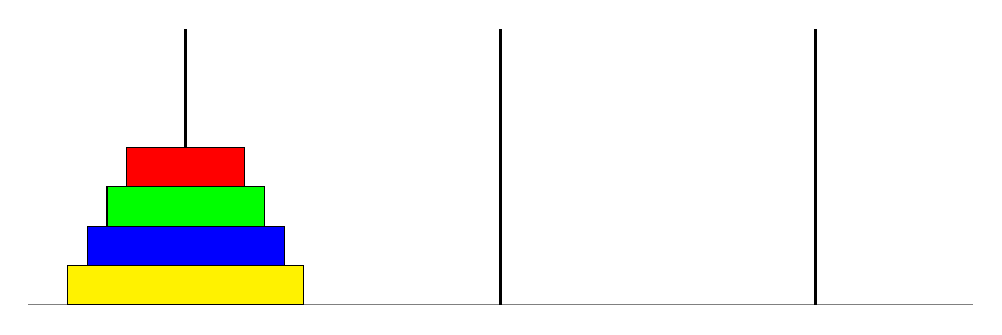
\begin{tikzpicture}[scale=0.5]
		\draw[-, gray] (0,0) -- (24,0);
		\draw[-, very thick] (4,0) -- (4,7);
		\draw[-, very thick] (12,0) -- (12,7);
		\draw[-, very thick] (20,0) -- (20,7);

		\draw[fill=red] (2.5,3) rectangle (5.5,4);
		\draw[fill=green] (2,2) rectangle (6,3);
		\draw[fill=blue] (1.5,1) rectangle (6.5,2);
		\draw[fill=yellow] (1,0) rectangle (7,1);
	\end{tikzpicture}
	\caption{汉诺塔}
\end{figure}

递归算法求解汉诺塔问题:

\begin{enumerate}
	\item 将n-1个圆盘从A借助C移到B。
	\item 将第n个圆盘从A移到C。
	\item 将n-1个圆盘从B借助A移到C。
\end{enumerate}

\vspace{-0.5cm}

\begin{lstlisting}[language=Python]
move = 0

def hanoi(n, src, mid, dst):
	global move

	if n == 1:
		print(src, "->", dst)
		move += 1
	else:
		# move top n-1 disks from src to mid
		hanoi(n - 1, src, dst, mid)
		print(src, "->", dst)
		move += 1
		# move top n-1 disks from mid to dst
		hanoi(n - 1, mid, src, dst)

def main():
	hanoi(3, "A", "B", "C")
	print("Moves:", move)

if __name__ == "__main__":
	main()
\end{lstlisting}

\begin{tcolorbox}
	\mybox{运行结果}
	\begin{verbatim}
A -> C
A -> B
C -> B
A -> C
B -> A
B -> C
A -> C
Moves: 7
	\end{verbatim}
\end{tcolorbox}

假设每次移动花费1秒,解决一个64层的汉诺塔问题大约需要5800亿年。\\

\begin{figure}[H]
	\centering
	
\includegraphics[]{img/Chapter5/5-4/2.png}
\end{figure}

\newpage